\documentclass{article}
\usepackage[top=2cm, bottom=2cm, left=2cm, right=2cm]{geometry}
\usepackage[english]{babel}
\usepackage{titling}
\usepackage{graphicx}
\usepackage[usenames,dvipsnames]{xcolor}
\usepackage{scrextend}
\changefontsizes[20pt]{12pt}
\usepackage{floatrow}
\usepackage{courier}
\usepackage{caption}
\usepackage{fontspec}
\setmonofont{DejaVu Sans Mono}
\title{Paper 2014 - A talk about Network}
\author{Daniel Maxime (Group 2326)}
\date{August 2014}

\begin{document}
\maketitle
\newpage

\tableofcontents
\clearpage

%
% Like most people we, English lecturers, use computer networks every day.
% We have a vague understanding of what IP addresses are, but what do they refer to exactly?
% There has been a lof a talk about IPv4, IPv6 and even IPv8 more recently.
% What are they? What are the differences?
% 
% Why do we need to mention « ports » in addition to « addresses » ?
% What’s the link between such « ports » and the notion of « service » ?
% Could you give some common examples ?
% 
% Last time we inadvertently opened a network configuration window,
% we came across the word "subnet mask": what is is, and what is it used for?
% 
% Is the subnet mask anything to do with routers?
% Isn't a router a computer ? Or is it the same as a switch?
%


\section{Introduction}
	\subsection{Computers network}
	
	Computers that we all know are useful for a lot a things: manage works, compute for science research,
	make movies, graohics, play games, ... But computers are more usefull when then can communicate with other !
	On top of all that, they can connect their users between them. That's probably the most important part of a
	computer nowadays. Interacting with computers is usefull but using it remotly or contacting services which
	is on the other side of the earth, it's just beautiful.
	
	The computer networks have undergone major changes over time. Multiple projects came out and
	only some of them (a single one in fact) survived. Let's see how this works...
	
	\subsection{A brief history}
	
	At first, to communicate with a computer system, you need a common way to "talk" with the others. To achieve
	this, some projects were made to try to unify the system with performance and well minded.
	
	The communication schema and definition (most of the time, this is public and accessible freely, under what we
	call, some RFC (Request For Comments)) used on computer science are call "Protocols".
	Some of them were made to connect computers between them: ARCnet, Ethernet, Token Ring, IP, ...
	
	These protocols were made for the same purpose (connect physically and logically devices) but with differents
	working method, the main difference is the way "how and when devices can talk".
	ARCnet and Token Ring uses "tokens" to allow someone to talk or not, Ethernet (which is the most used now)
	talk when he want and manage collisions (when two people talk on the same time).
	
	I'll only keep protocols which are still used nowadays, everywhere, and skip the others.
	But, how these protocols works togethers ?

\section{Network layers}

	The perk of the network base is the "OSI model" (Open Systems Interconnection model) which characterizes and
	standardizes the internal functions of a communication system. All "internet" network uses it. This model split
	the works with 7 layers, each independant of one another. You can changer a layer without affecting the content
	of the others. It's due to this method that you can browse the web on wireless or wired connection, without change
	all your hardware.
	
	Let me explain these layers from the bottom to the top, to understand how each small protocol used on internet
	works together to provide a full and flexible support. After that, we will see how theses protocols interacts
	with others.
	
	\subsection{Layer 1 - Physical layer}
	
	This layer is definitively the easiest layer of the OSI model, it's globally just the wire which connect one
	device to another (your computer to your Internet Provider's box, the Internet Provider's box to their
	data center, etc). In your house, except "ethernet-cable" or wireless access, you probably don't have
	any other layer 1 technology, but there are many other.
	
	Now, we have a cable between two devices, that's fine, but how can I make it communicate ?
	With the layer 2 of course.

	\subsection{Layer 2 - Data link layer}
	
	This (single) layer permits to devices to communicate together, on a small area (eg: devices you have at your house,
	nothing more). The most common protocol used at this layer is Ethernet. This protocol is made to tramsit data
	over the layer 1, with some collisions and errors detection. After that, to connect two devices bewteen them, you
	need to use addresses. Ethernet use MAC addresses.
	\footnote{No, you don't need to have an "Apple Mac Computer" to have a MAC address.
	All physical ethernet network cards got a unique one on the world.}
	\footnote{Exemple of MAC address: 00:54:77:65:78:21}
	A MAC address is 48 bits longs, that's means that there are about 281,000 billion address possible. I think that's
	suffisant for your home (yes, remimber, this protocol connects only a small area).
	
	This protocol, like all protocols (you will see later) use a generic data representation:
	header + payload (+ footer).
	The footer is not always present on protocols, but often, this is where is put "checksum" (a small amount of data
	wihich enables corruption detection).
	
	The header is dedicated for Ethernet, the payload is simply used to put
	the layer 3 on it. This method is called "encapsulation" (like Matriochka), it's with this method that all layers
	will be put together.
	
	To communicate with someone, we must know it's address, but when we talk to someone, it's a good idea to
	get it's response. To help it to respond, we will provide our address too. Well, the header will contains
	at least the destination address and the source (our) address. This will be the same for all protocols
	that we'll see.
	
	Now we can connect two devices and exchanges data (on the payload) between them. Let's see how we can extends
	the area of communication (internet on your home only it's not very interresting).
	
	\subsection{Layer 3 - Network layer}
	
	To extends your connectivity all around the world, using MAC address only is not possible due to conception
	on the protocol: ethernet, as I said is made for local traffic. To extends this traffic to the outside, we need
	to use another protocol, which is made for that. We called IP (Internet Protocol). Yes, this is really the protocol
	which is really used to have "Internet".
	
	Nice, but, what is IP exactly ? IP is the protocol which permits to make the link with the underlaying layer
	and global mapped address. IP uses... IP address
	\footnote{Exemple of IP address: 82.212.175.9} to represents source and destination. For the v4 of the protocol
	(commonly called IPv4), address are 32 bits long, which make about 4 billions unique address. For the begening of
	the "Internet time", this was absolutly huge.
	
	One more time, we will encapsulate this protocol on the underlaying protocol. We have this schema right now:
	\begin{center}
	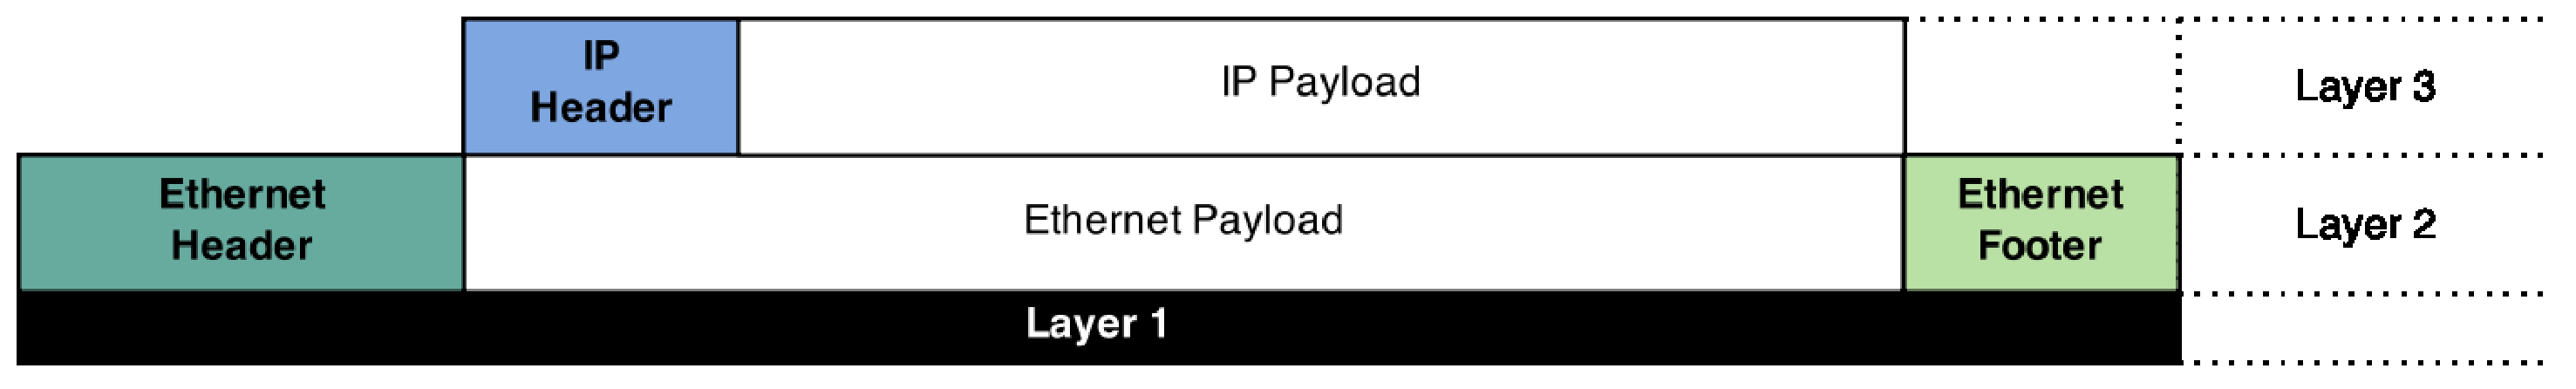
\includegraphics[scale=0.3]{content/layer3.eps}
	\end{center}
	
	We can now contact devices outside our home. We will see later how and why it's only now that we can contact
	the "outside world". But that's nice, but how can I contact a specific service (web browser, file transfert, chat, ...)
	on a specific device, we only know it's address right now.
	
	\subsection{Layer 4 - Transport layer}
	
	To understand un little bit more how that's works, I'll draw an analogy with real life. Imagine a world with
	road and a lot of buildings with flats. Roads it's the layer 1 (wire), your car is layer 2 (etnernet), the building
	address, flat stage and flat number is described by the IP address. Now you are at your destination, you want to
	go to a specific location on this flat. When your enter the flat, you are in the lobby, you have multiple doors
	in front of you. That's the solution. Behind each doors you have one service.
	
	Theses doors on network are called "ports".
	
	This happen on layer 4 with multiple possibe protocols. The most used are TCP and UDP. They are both the same purpose
	and differents ports, but works in two way differents, these way are not important to understand how it works.
	
	Just keep in mind that these ports enable you to access specific services on the remote device. Like each time,
	this works with encapsulation. That's what we have after this encapsulation:
	\begin{center}
	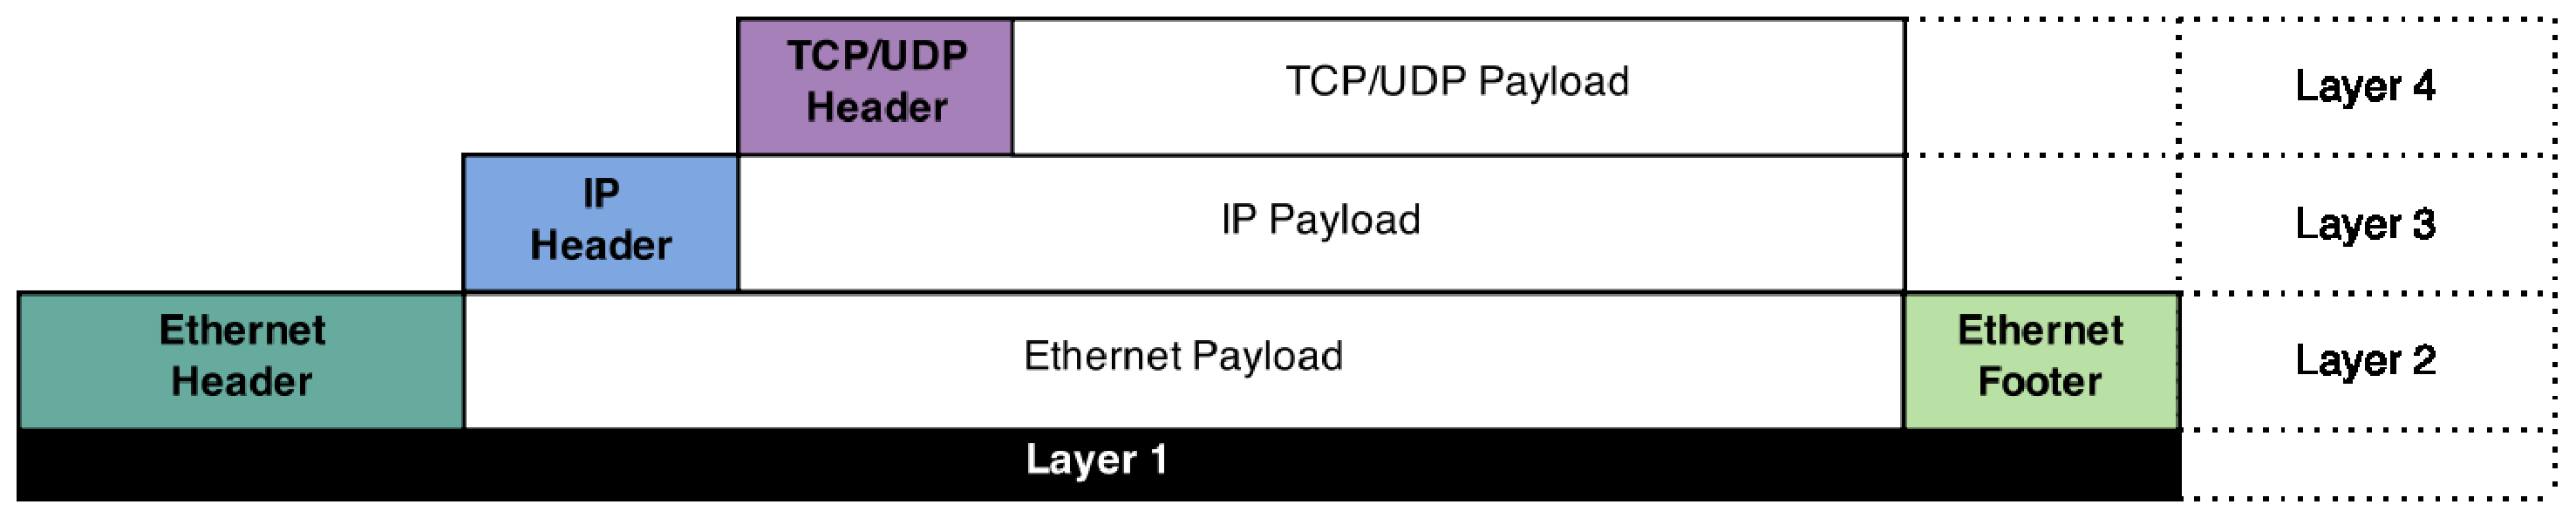
\includegraphics[scale=0.3]{content/layer4.eps}
	\end{center}
	
	Like before, the header contains the source port and the destination port. Yes, you have a source port. In fact,
	a webserver is a service behind a door, but your web browser is a service too, behind a door at your home.
	That's explain how you can browser multiple differents website at the same times: everythings has it's own door (port).
	
	And voila. You can communicate and exchange data with your correspondant ! But, what kind of data ?
	
	\subsection{Layer 7 - Application layer}
	
	We are now at layer 7. What ? And what about layer 5 and 6 ? They are not important for us, we can skip it, most
	of the times, these layer are not used at all because we don't need them.
	
	Well, what's is the layer 7 ? It's simply data you want to exchange. You can send "hello" (really just "hello"),
	and that's what the remote service (remember, door) will receive. That's easy but, to request a web page for exemple,
	we must provide a comprehensive way to talk with the web server. To perform that's correctly, we use... one more time,
	protocols ! At this layer, we found a lot of protocols: http, ftp, ssh, irc, telnet, smtp, pop3, imap, ...
	
	Each of these protocols have a default port number. The exact content of the protocol is describe on each RFC
	specially written for that.
	
	Now, our complete frame look like that:
	\begin{center}
	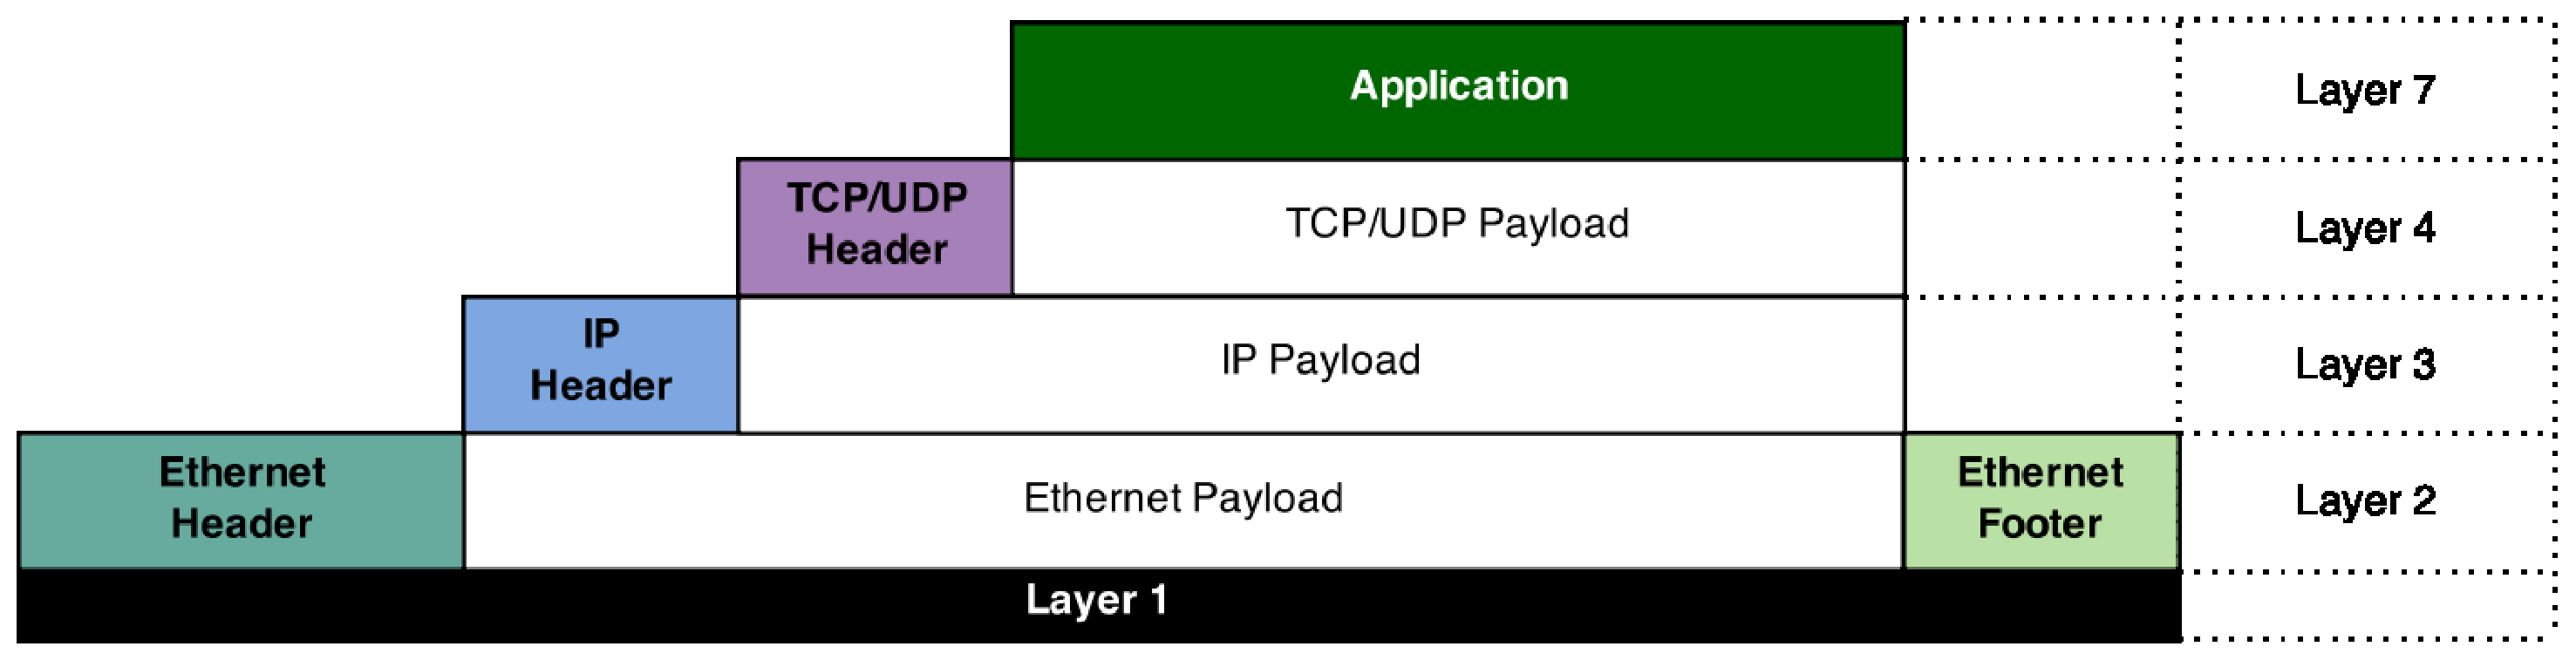
\includegraphics[scale=0.3]{content/layer7.eps}
	\end{center}
	
	That's nice, but why do we need all of these protocols to reach the wanted destination, and why have we split that ?
	To understand that's, we must go deeper in the description.

\section{A little deeper...}
	You have (I hope) the schema with building, flats and roads on your mind. Keep it fresh, I'll complete it to well
	understand some devices and specific additionnal services you can find on networks.
	
	For specific reasons, flats can communicate with layer 2 with the same floor only (you have probably 3 or 4 flats
	per stages). To communicate between flats, we need to connect them to each other, for that we will use a "switch".
	This device's job is just to send traffic (based on destination MAC address) on the right wire connected.
	
	To communicate with your building (without go outside your building I mean), you need to connect each stages between
	them. You can use switch to connects each switch between them (that's pretty easy no ?). Each flat has it's own
	IP address, and to segments all the Internet IP Address, we will split it per building. Each building has it's own
	part of "The Internet (IP)". This part is called "subnet". With this feature, you can communicate with your building
	without additionnal devices or something else. You are isolated.
	
	To make building communucate with others, you need to put a device on the building door, which will works on the
	link between the building and the road. To access some roads and know which road take, we use a devices
	which know these road... or more precisely, these routes ! These devices are called... router. Easy not ?
	
	The job of a router is just to connect your sub-network with others.
	
	One interresting thing that we can put on the building too, is a security agent. We can put one on the router, to
	control who enter and go out the building, and we can put a security agent on each flat, to control who comes in, 
	trying to access some services. If this security agent see someone not autorised, it will simply throw it out.
	This security agent is called "firewall".
	
	That's all folk ! You now know basiclly how a computer network works. Pretty simple, no ? That's how it works
	nowadays, but computer science is a science which progress each days, and the futur is already concidered.

\section{What's next ?}
	Remember you, I explained you layer 3 with "IP" version 4 (IPv4). Nowadays, IPv6 exists. In fact, IPv4 with it's
	32 bits long for address is too short now. We are really close to reach the limit of existing address, that's the
	main reason for IPv6 to exists. The main new think that IPv6 improve is the address no more on 32 bits,
	but on 128 bits. That put the limits at about approximately 3.4x$10^{38}$ addresses. This is really really big.
	This is not the only one change with IPv6, some technical details changes too. IPv4 is more than 30 years old, 
	since this time, we found and improved IPv6 with some missing or some deprecated features.
	
	To enable everyone to have IPv6 at their home, the world must use a software IPv6-capable. But the avantage of
	layerd system is that we must only change layer 3 of the whole system, the other layers remain unchanged. That means
	that HTTP, TCP and Ethernet still works the same way on IPv4 or IPv6. That's so beautiful !
	
	Finally, if you heard of IPv8, IPv9 or something like that, forget it, they doesn't exists. Simply.

\section{Conclusion}
	You now know how computers networks (Internet mainly) works, with which protocols and how they communicate each other.
	Your network cards contains a MAC address used by IP to go outside your house. You have ports which specify service
	and the application protocol which contains your requests for specific services.
	
	\newpage

\section{Sources}
	\begin{itemize}
		\itemsep0em
		\item https://en.wikipedia.org/wiki/Ethernet
		\item https://en.wikipedia.org/wiki/Internet\_Protocol
		\item https://en.wikipedia.org/wiki/MAC\_address
		\item https://en.wikipedia.org/wiki/ARCnet
		\item https://en.wikipedia.org/wiki/TokenRing
		\item https://en.wikipedia.org/wiki/OSI\_model
		\item Graphics are made using https://draw.io
	\end{itemize}
	
\end{document}







